\chapter{Background}
\label{chap:background}

\section{Background}
Based on the previous work of people using NSGA-II on some multi-objective optimization problems\cite{Magnier_2010_Multiobjective}, NSGA-II could also apply for Urban Design optimization problem. 

\section{Previous Work}

% \subsection{Genetic Algorithm(GA)}
The idea of Genetic Algorithm(GA) was from Darwin's Theory of Evolution and was first invented by John Henry Holland in 1975\cite{Holland_1975_Book}. Mimicking the process of natural selection, GA uses selection, crossover, and mutation operations to generate solutions and tries to find the optimal solution. More specifically, an initial random population is given at the beginning. Then based on criterions or objectives, each individual is assigned a fitness value. After selecting a certain number of individuals from the initial population based on their fitness values, crossover operation with a crossover probability is applied on those individuals to generate some new offspring. Next, mutation operation with a mutation probability is applied on the new offspring. After all those steps, hopefully it can give us a new population which have some individuals with better fitness values. Last, consider this output population as the new initial population and repeat selection, crossover and mutation operations until pareto optimal solutions are achieved. After this framework was constructed, it has been used in many areas, such as Artificial Intelligence, Bioinformatics, Building Design, Scheduling Problems, etc. While, on the way to solve practical problems, people have put a lot of effort to improve GA. Next, some of those milestone variations of GA will be shown.

\subsection{Multiobjective Genetic Algorithm(MOGA)}
In general, optimal problems could be divide into two categories based on the number of objectives: Single Objective problems and Multi-Objective problems. In order to understand MOGA, a toy example is necessary. A simple example of a single objective problem is to find the minimum value of \(y=x^2\) with \(x\in [-3,3]\). Clearly, the minimun value could be achieved at \(x=0\), \(y=0\). However, when there are two objectives, the problem becomes more complicated. For example, instead of just minimizing \(y=x^2\), both \(y_{1}=x^2\) and \(y_{2}=(x-2)^2\) want to be minimized. Then, there is not a specific \(x\) value for this problem. \autoref{fig:two_functions} shows us \(x\) at 0 could achieve minimum value of \(y_{1}=x^2\) and \(x\) at 2 could achieve minimum value of \(y_{2}=(x-2)^2\). However, there is no \(x\) value which could guarantee both \(y_{1}\) and \(y_{2}\) at their minimun value. For \(x=\) \(0\) or \(2\), people usually call them Pareto Optimal Solutions\cite{Hans_1988_Multicriteria_Pareto_Optimal}\cite{Vira_1983_Multiobjective_Pareto_Optimal}. Other than \(x=\) \(0\) or \(2\), any points between \(0\) and \(2\) could be a valid compromise solution. 

\begin{figure}[htp] 
\centering
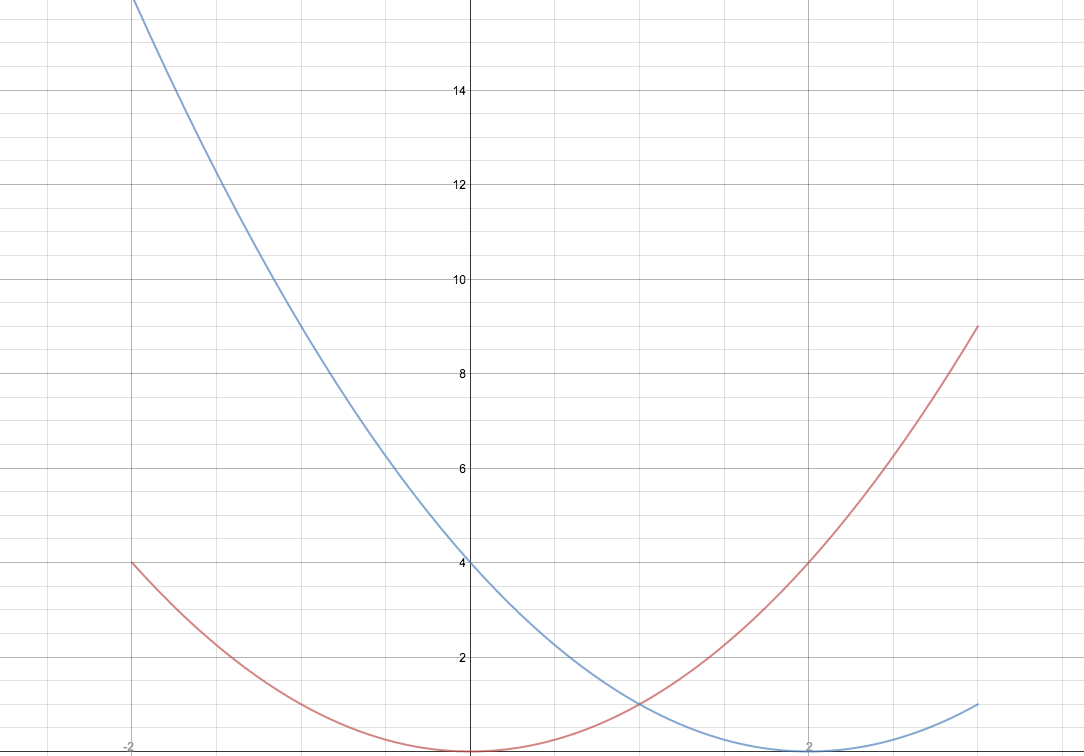
\includegraphics[scale=.2]{images/Figure_1.png}
\caption{Functions \(y_{1}=x^2\) and \(y_{2}=(x-2)^2\)}
\label{fig:two_functions}
\end{figure}

In the real world, there are many kinds of simultaneous optimization of multiple objectives. People have tried many methods to find Pareto Optimal Solution. The classical method is to convert a multiobjective problem to a single objective problem. In paper \cite{NSGA_1994}, three classical methods are introduced: 1.Objective Weighting, 2.Distance Functions, and 3.Min-Max Formulation. All those methods have one common drawback: they can only give us a single-point solution. However, when people make decisions, they often need different alternatives. Another significant drawback of those methods is they heavily depend on what weight vector or demand level chosen, which requires that the user have knowledge about the underlying problem. However, in most cases, users do not have much knowledge about the problem and that is one of the reasons they use genetic algorithm. So, those methods are not efficient and users probably need to try many times to get an acceptable solution.

Since classical methods to solve multiobjective optimization problems are inadequate and inconvenient, people started to find other ways to implement GA.

\subsection{Vector Evaluated Genetic Algorithm(VEGA)}
VEGA is the first practical algorithm and was developed by Schaffer in 1984\cite{Schaffer_1984_Some}. Instead of changing a multiple objective problem to a single objective problem, Schaffer modified the simple tripartite genetic algorithm by performing independent selection cycles according to each objective\cite{Schaffer_1984_Some}. Bascially, to fill up a portion of the mating pool, he created a loop around the traditional selection procedure to repeat selection method for each individual objective. After this selection step, we could have a thoroughly shuffled population to apply crossover and mutation steps. This could make the mating of individuals from different subpopulation groups possible.

With the independent selection of specialists, we could make the population in speciation. After a large number of generations, we could see the convergence of the entire population toward the individual optimum regions. To make a decision, we may not want to have any bias on such middling individuals, rather, we desire more nondominated points. Schaffer developed two heuristics to minimize this speciation: the nondominated selection heuristic and the mate selection heuristic. For the nondominated selection heuristic, he penalized the dominated individuals by substracting a small fixed penalty from their expected number of copies druing selection. Then the total penalty for dominated individuals was divided among the nondominated individuals and was added to their expected number of copies during selection. For the mate selection heuristic, he wanted to promoted the cross-breeding of specialists from different subgroups by selecting an individual, as a mate to a randomly selected individual, which has the maximum Euclidean distance in the performance space from its mate. However, both of those two heuristics are failed due to some certain problems.

Overall, VEGA could solve the drawback in the classical MOGA and give us multiple Pareto Optimal Solutions without depending on the weight or demand level. But, in some cases it suffered from its bias toward some individuals or regions. After that, people tried many other methods to avoid the bias.

\subsection{Nondominated Sorting Genetic Algorithm(NSGA)}
NSGA was first introduced by N. Srinivas and Kalyanmoy Deb in 1994\cite{NSGA_1994}. They investigated Goldberg's notion of nondominated sorting in GAs along with a niche and speciation method to find multiple Pareto Optimal Solutions simultanesously. The reason they call this algorithm the Nondominated Sorting Genetic Algorithm is that it build on a nondominated sorting procedure. Two ideas behind the nondominated sorting procedure are ranking selection which is used to emphasize good points method and niche method which is used to maintain stable subpopulations of good points.

The only difference between simple genetic algorithm and NSGA is the way selection operator works. First, we rank the population based on the individuals' nondomination and identify those nondominated individuals from the current population. Second, let all those individuals constitute the first nondominated front and assign a large dummy fitness value to them. All those nondominated individuals which have an equal reproductive potential should have same fitness value. Third, to maintain diversity in the population, we apply sharing methods\cite{Deb_1989_Investigation}\cite{Deb_1989_Genetic} on these classified individuals. Sharing is achieved by performing selection operation using degraded fitness values that are obtained by dividing the original fitness value of an individual by a quantity proportional to the number of individuals around it. Last, ignore those nondominated multiple optimal points and using the same method to process the rest of population to get the second nondominated front. This time, we assign a new dummy fitness value to the second nondominated front which is smaller than the first nondominated front. By this process, we could classified the entire population into several fronts. After the classification process, we reproduct the population by each individual's dummy fitness value and apply a stochastic remainder proportionate seletion on them.

After this selection process, we move to crossover operation. Since we want to find nondominated regions or Pareto Optimal fronts and first front have the maximum fitness value, we give them more copies. This could give us a fast convergence of the population toward nondominated regions. Furthermore, sharing method could help us to distribute the population over this region. By nondominated sorting procedure, NSGA becomes faster than VEGA. And NSGA can solve both minimization and maximization problems. However, it is still not very convenient. We still need to specify the sharing parameter and it is lack of elitism.

\subsection{Nondominated Sorting Genetic Algorithm II(NSGA-II)}
In 2002, Kalyanmoy Deb, Amrit Pratap, Sameer Agarwal, and T. Meyarivan made some modification on NSGA to upgrade it to NSGA-II\cite{NSGA_II}. After NSGA-II was introduced, it has been used in many area, such as Building Design\cite{Magnier_2010_Multiobjective}, Hydro-Thermal Power Scheduling\cite{Deb_2007_Dynamic}, Soil and Water Assessment Tool\cite{Bekele_2007_Multi}, etc. Moreover, in our paper, we will use it to solve Urban Design problem. 

Compare with the previous NSGA, NSGA-II has improved the computational efficiency, elitism, and sharing parameter\cite{NSGA_II}. For computational complexity of nondominated sorting, it improve from \(O(MN^{3})\) to \(O(MN^{2})\) by using fast nondominated sorting approach\cite{NSGA_II}. With the elitism, NSGA-II could not only speed up the GA performance, but also prevent loss of good solutions. Moreover, NSGA II does not need to specify a sharing parameter \(\sigma_{share}\), which is a requirement for pervious multi-objective evolutionary algorithms. Instead of using sharing function approach, NSGA-II is using Crowded-Comparison Operator, which could both improve the computational complexity and maintation a spread of solutions.

% \subsection{Pareto Optimal Solution}

